\chapter{النمذجة الحركية (\LR{Kinematic Modeling})}
\label{ch:kinematics}

يعتبر النموذج الحركي الخطوة الأولى والأساسية في تحليل أي مناور روبوتي. يهتم هذا الفصل بدراسة حركة الروبوت من منظور هندسي صرف دون التطرق إلى القوى أو العزوم المسببة لهذه الحركة. من خلال الاعتماد على المعطيات الهندسية لأطوال الوصلات وحدود حركة المفاصل، سيتم بناء النموذج الحركي المباشر الذي يربط بين إحداثيات المفاصل الداخلية للروبوت والموضع الفراغي الديكارتي للمؤثر النهائي، وهو ما يعتبر ضرورياً لمعرفة النطاق التشغيلي للذراع وتقييم مساراتها الفراغية لاحقاً.


\section{تعيين المحاور الإحداثية (\LR{Coordinate Frames Assignment})}
\label{sec:frames}

الخطوة الأولى في خوارزمية دينافيت-هارتنبيرغ (\LR{DH}) هي ربط جملة إحداثيات ديكارتية محلية بكل وصلة من وصلات الروبوت، بدءاً من القاعدة الثابتة (\LR{Base}) وصولاً إلى المؤثر النهائي. بالنسبة للروبوت (\LR{SCARA}) المدروس، تم توجيه المحاور وفق القواعد الهندسية التالية:

 \begin{figure}[H]
     \centering
     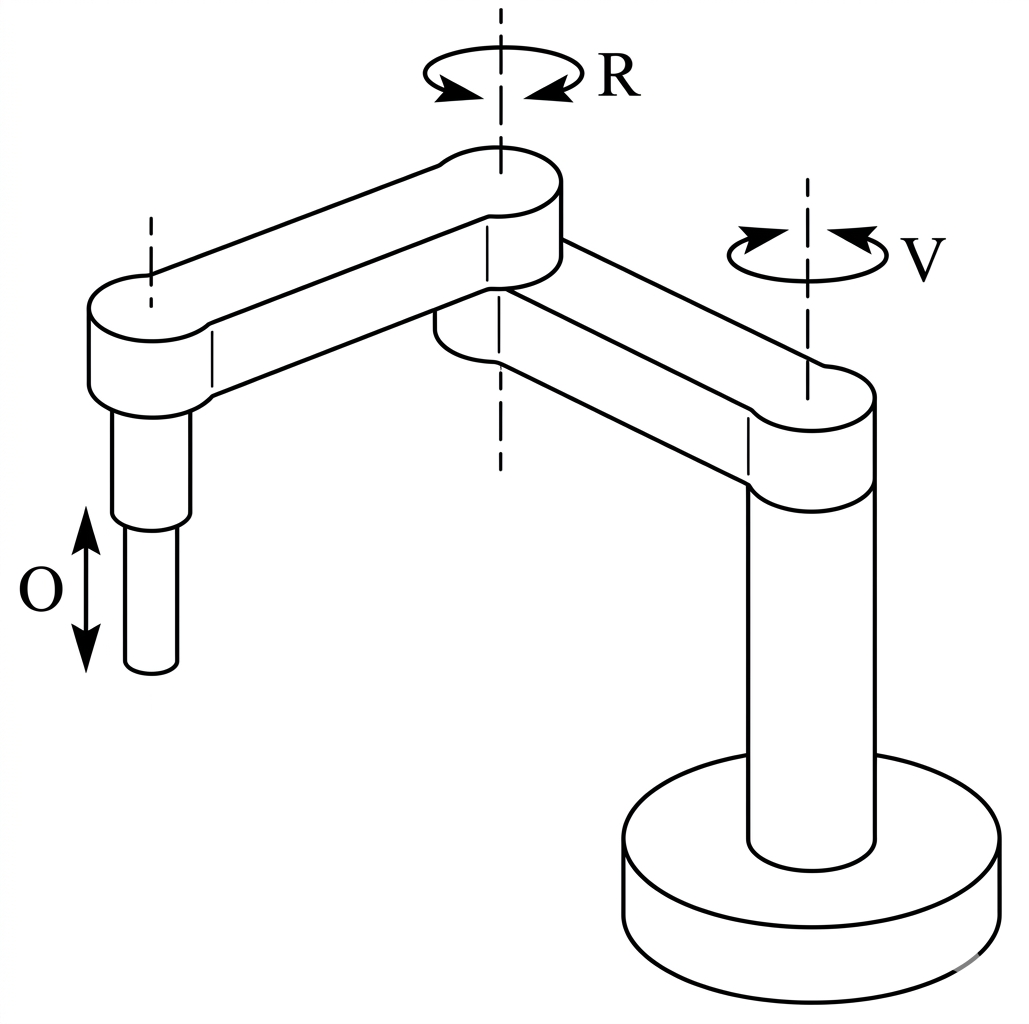
\includegraphics[width=0.7\textwidth]{resources/images/scara_arm}
%     \caption{توزيع المحاور الإحداثية على مفاصل الروبوت وفق خوارزمية \LR{DH}}
     \label{fig:frames}
 \end{figure}

\begin{itemize}
    \item \textbf{المحاور $Z_0$ و $Z_1$:} تم توجيهها عمودياً على المستوي الأفقي لتمثل محاور الدوران للمفصلين الأول والثاني.
    \item \textbf{المحور $Z_2$:} يمثل محور الحركة الانسحابية للمفصل الثالث، وتم توجيهه نحو الأسفل (باتجاه منطقة العمل).
    \item \textbf{المحاور $X_i$:} تم توجيهها على امتداد الوصلات الميكانيكية (\LR{Links}) بحيث تكون عمودية على المحور $Z_{i-1}$ وتتقاطع معه.
\end{itemize}


\section{  \LR{DH table}}
\label{sec:dh_table}

بناءً على التوزيع الهندسي لجمل الإحداثيات الموضحة في القسم السابق، يتم استخراج المعاملات الأربعة الخاصة بخوارزمية (\LR{DH}) لربط كل جملتين متتاليتين ($i-1$) و ($i$). تُعرّف هذه المعاملات الأربعة كما يلي:
\begin{itemize}
    \item $a_i$: الإزاحة الخطية على طول المحور $X_i$ من المحور $Z_{i-1}$ إلى المحور $Z_i$.
    \item $\alpha_i$: الإزاحة الزاوية (الفتل) حول المحور $X_i$ من المحور $Z_{i-1}$ إلى المحور $Z_i$.
    \item $d_i$: الإزاحة الخطية على طول المحور $Z_{i-1}$ من المحور $X_{i-1}$ إلى المحور $X_i$.
    \item $\theta_i$: الإزاحة الزاوية حول المحور $Z_{i-1}$ من المحور $X_{i-1}$ إلى المحور $X_i$.
\end{itemize}

بتطبيق هذه القواعد على البنية الميكانيكية للروبوت المدروس (\LR{SCARA})، تم استنتاج الوسطاء الحركية للمفاصل الثلاثة كما هو موضح في الجدول (\ref{tab:dh_parameters}). 

\begin{table}[H]
    \centering
    %\caption{DH table}
    \label{tab:dh_parameters}
    \renewcommand{\arraystretch}{1.5}
    \begin{tabular}{|c|c|c|c|c|c|}
        \hline
        \textbf{المفصل ($i$)} & \textbf{نوع المفصل} & \textbf{$\theta_i$} & \textbf{$d_i$} & \textbf{$a_i$} & \textbf{$\alpha_i$} \\
        \hline
        1 & دوراني (\LR{Revolute}) & $\theta_1$ & $0$ & $L1$ & $0$ \\
        \hline
        2 & دوراني (\LR{Revolute}) & $\theta_2$ & $0$ & $L_2$ & $180^\circ$ \\
        \hline
        3 & انسحابي (\LR{Prismatic}) & $0$ & $d_3$ & $0$ & $0$ \\
        \hline
    \end{tabular}
  
 
\end{table}


\section{\LR{Homogeneous Transformation Matrices}}

\label{sec:transformation}

تمثل مصفوفة التحويل المتجانس أداة رياضية قوية تدمج بين الدوران (\LR{Rotation}) والانسحاب (\LR{Translation}) في مصفوفة واحدة بأبعاد $4 \times 4$. تُعطى المصفوفة العامة للتحويل المتجانس \LR{$A_i^{i-1}$}، التي تنقل الإحداثيات من الجملة \LR{($i$)} إلى الجملة \LR{($i-1$)} وفق خوارزمية (\LR{DH})، بالعلاقة الرياضية التالية:

\begin{equation}
A_i^{i-1} = 
\begin{bmatrix}
\cos\theta_i & -\sin\theta_i \cos\alpha_i & \sin\theta_i \sin\alpha_i & a_i \cos\theta_i \\
\sin\theta_i & \cos\theta_i \cos\alpha_i & -\cos\theta_i \sin\alpha_i & a_i \sin\theta_i \\
0 & \sin\alpha_i & \cos\alpha_i & d_i \\
0 & 0 & 0 & 1
\end{bmatrix}
\label{eq:general_dh}
\end{equation}

لإيجاد مصفوفات التحويل الخاصة بمفاصل الروبوت المدروس، نقوم بتعويض المعطيات المستخرجة في الجدول (\ref{tab:dh_parameters}) داخل المعادلة العامة (\ref{eq:general_dh}). ولتبسيط الكتابة الرياضية، تم اعتماد الاختصارات المثلثية المعيارية حيث \LR{$c_i = \cos\theta_i$} و \LR{$s_i = \sin\theta_i$}.

\textbf{1. التحويل من الجملة \{1\} إلى الجملة \{0\}:}
بتعويض بارامترات المفصل الأول، حيث \LR{$d_1 = 0$}، و \LR{$a_1 = L_1$}، و \LR{$\alpha_1 = 0$}، وبما أن \LR{$\cos(0) = 1$} و \LR{$\sin(0) = 0$}، نجد:

\begin{equation}
A_1^0 = 
\begin{bmatrix}
c_1 & -s_1 & 0 & L_1 c_1 \\
s_1 & c_1 & 0 & L_1 s_1 \\
0 & 0 & 1 & 0 \\
0 & 0 & 0 & 1
\end{bmatrix}
\label{eq:A10}
\end{equation}

\textbf{2. التحويل من الجملة \{2\} إلى الجملة \{1\}:}
بتعويض بارامترات المفصل الثاني، حيث \LR{$d_2 = 0$}، و \LR{$a_2 = L_2$}، و \LR{$\alpha_2 = 180^\circ$}، وبما أن \LR{$\cos(180^\circ) = -1$} و \LR{$\sin(180^\circ) = 0$}، تتغير إشارات بعض العناصر لنحصل على:

\begin{equation}
A_2^1 = 
\begin{bmatrix}
c_2 & s_2 & 0 & L_2 c_2 \\
s_2 & -c_2 & 0 & L_2 s_2 \\
0 & 0 & -1 & 0 \\
0 & 0 & 0 & 1
\end{bmatrix}
\label{eq:A21}
\end{equation}

\textbf{3. التحويل من الجملة \{3\} إلى الجملة \{2\}:}
بتعويض بارامترات المفصل الانسحابي الثالث، حيث \LR{$\theta_3 = 0$}، و \LR{$a_3 = 0$}، و \LR{$\alpha_3 = 0$}، تنتج لدينا مصفوفة تمثل انسحاباً خطياً نقياً على المحور \LR{$Z$}:

\begin{equation}
A_3^2 = 
\begin{bmatrix}
1 & 0 & 0 & 0 \\
0 & 1 & 0 & 0 \\
0 & 0 & 1 & d_3 \\
0 & 0 & 0 & 1
\end{bmatrix}
\label{eq:A32}
\end{equation}
\section{معادلات الموضع الديكارتي (\LR{Cartesian Position Equations})}
\label{sec:position}

للحصول على التحويل الفراغي الكلي من قاعدة الروبوت إلى نقطة المؤثر النهائي، يتم ضرب مصفوفات التحويل المتسلسلة التي تم حسابها في القسم السابق ببعضها البعض:

\begin{equation}
T_3^0 = A_1^0 \cdot A_2^1 \cdot A_3^2
\end{equation}

وبعد إتمام عمليات الضرب المصفوفي وتطبيق متطابقات المجموع للزوايا المثلثية، تم التوصل إلى مصفوفة التحويل الكلية \LR{$T_3^0$}. ولتبسيط عرض المصفوفة، تم استخدام الاختصارات \LR{$c_{12} = \cos(\theta_1 + \theta_2)$} و \LR{$s_{12} = \sin(\theta_1 + \theta_2)$}:

\begin{equation}
T_3^0 = 
\begin{bmatrix}
c_{12} & s_{12} & 0 & L_1 c_1 + L_2 c_{12} \\
s_{12} & -c_{12} & 0 & L_1 s_1 + L_2 s_{12} \\
0 & 0 & -1 & -d_3 \\
0 & 0 & 0 & 1
\end{bmatrix}
\end{equation}

يمثل العمود الرابع من هذه المصفوفة شعاع الموضع الديكارتي للمؤثر النهائي في الفضاء التشغيلي. ومنه، يمكن استخلاص معادلات الحركة المباشرة النهائية \LR{($x, y, z$)} بدلالة الإحداثيات المفصلية \LR{($\theta_1, \theta_2, d_3$)} وأطوال الوصلات \LR{($L_1, L_2$)} كما يلي:

\begin{equation}
\begin{cases}
x = L_1 \cos(\theta_1) + L_2 \cos(\theta_1 + \theta_2) \\
y = L_1 \sin(\theta_1) + L_2 \sin(\theta_1 + \theta_2) \\
z = -d_3
\end{cases}
\label{eq:fk_position}
\end{equation}
يُلاحظ من المعادلة الأخيرة أن الإحداثي $(z)$ يأخذ قيمة سالبة $(-d_3)$، وهذا يتوافق رياضياً وفيزيائياً مع البنية الميكانيكية، حيث أن المحور $Z_2$ موجه نحو الأسفل، وبالتالي فإن الإزاحة الموجبة للمفصل الانسحابي ستؤدي إلى نزول الذراع أسفل مستوي القاعدة المرجعية.